\documentclass{ta-its}
\usepackage{hyperref} % Hyperlink pada dokumen
\usepackage{listings} % Kode sumber

% \title{Judul Bahasa Indonesia}{Judul Bahasa Inggris}
\title{Rancang Bangun Sistem Load Balancing Menggunakan Algoritma Berbasis Konten dan Kontrol Ketersediaan Layanan}{Design and Implementasion of Load Balancing System with Content-Based Algorithm and Availability Control}{KI1502} 

% \author{Nama Lengkap}{NRP}
\author{Bahrul Halimi}{5111100014}

% \supervisorOne{Nama Pembimbing Satu}{NIP}
% \supervisorTwo{Nama Pembimbing Dua}{NIP}
\supervisorOne{Royyana Muslim Ijtihadie, S.Kom, M.Kom, PhD}{197708242006041001}
\supervisorTwo{Baskoro Adi P, S.Kom, M.Kom}{197708242006041001}

% \degree{Nama Gelar}{Bidang Studi}{Program Studi}{Jurusan}{Jurusan (English)}{Fakultas}{Fakultas Singkatan}{Fakultas (English)}
\degree{Sarjana Komputer}{Arsitektur dan Jaringan Komputer}{S1}{Teknik Informatika}{Informatics}{Teknologi Informasi}{FTIf}{Information Technology}

% \time{bulan}{tahun}
\time{Desember}{2015}

\begin{document}
    \frontmatter % Halaman dengan penomoran romawi kecil
    \maketitle
    \legalityPaper % Lembar Pengesahan
    \begin{abstrak}
    	Dokumen ini merupakan dokumen contoh penggunaan templat \LaTeX{} untuk pembuatan Buku Tugas Akhir ITS. \\
    	
    	\noindent \textbf{Kata-Kunci}: \LaTeX{}, templat, Tugas Akhir, ITS.
	\end{abstrak}
   \begin{abstract}
    	Dokumen ini merupakan dokumen contoh penggunaan templat \LaTeX{} untuk pembuatan Buku Tugas Akhir ITS. \\
    	
    	\noindent \textbf{Kata-Kunci}: \LaTeX{}, templat, Tugas Akhir, ITS.
	\end{abstract}
    \chapter{Kata Pengantar}
        \textbf{Om Swastyastu}

        Puji syukur penulis haturkan kepada Ida Sang Hyang Widhi Wasa, Tuhan Yang Maha Esa karena atas \emph{asungkertha wara nugraha} beliau, penulis dapat menyelesaikan sebuah dokumentasi cara pembuatan Buku Tugas Akhir Sarjana menggunakan \LaTeX{} untuk Institut Teknologi Sepuluh Nopember, Surabaya. Dokumentasi ini diharapkan dapat membantu rekan-rekan mahasiswa S1 yang menempuh semester terakhir dengan membuat buku Tugas Akhir menggunaan sistem \emph{typesetting} \LaTeX{} yang terbukti handal dan lumrah digunakan di bidang penelitian sains dan teknik. Dokumentasi ini dibuat menggunakan templat yang penulis buat sendiri (pada berkas \texttt{ta-its.cls}) sehingga nantinya bisa digunakan kembali sehingga pembuatan buku bisa lebih dipermudah.

        Penulis menerima kritik dan saran mengenai pengembangan templat ini agar bisa menjadi lebih baik dan bisa menjadi standar \emph{de-facto} dan \emph{de-jure} dalam penulisan buku TA di seluruh civitas akademika ITS. Penulis dapat dihubungi melalui surel: \texttt{initrunlevel0@gmail.com}.

        Sekian dan Terima Kasih.
        \noindent \textbf{Om Santhi Santhi Santhi Om}

        \cleardoublepage % Mengisi penanda halaman genap yang kosong

    \tableofcontents % Daftar isi
    \listoftables % Daftar tabel
    \listoffigures % Daftar figur/gambar

\mainmatter % Halaman utama, dengan judul BAB X, nomor halaman penomoran arab
    \chapter{PENDAHULUAN}
        Pada bab ini akan dipaparkan mengenai garis besar Tugas Akhir yang meliputi latar belakang, tujuan, rumusan dam batasan permasalahan, metodologi pembuatan Tugas Akhir, dan sistematika penulisan.

        \section{Latar Belakang}
            Semakin berkembangnya internet di masyarakat membuat penggunaan aplikasi berbasis web semakin diminati. Pengguna aplikasi berbasis web ini dapat dijumpai diberbagai aktivitas harian masyarakat, diantaranya bank \emph{online}, \emph{e-commerce}, reservasi tempat secara \emph{online}, bahkan pendaftaran peserta didik baru secara \emph{online}. Hal ini membuat penyedia layanan aplikasi berbasis web harus menyediakan servis yang layak sehingga aplikasi tetap berjalan dengan baik walaupun pengguna semakin bertambah.\\

\indent Terjadinya bottleneck (penumpukan permintaan) menjadi tantangan tersendiri ketika pengembang tidak memperhatikan sumber dayanya dan berujung pada gagalnya permintaan pengguna [1]. Muncul gagasan awal dengan penggunaan kelompok server yang akan menangani permintaan ini. Kelompok server ini akan secara bergantian melayani setiap permintaan terhadap aplikasi berbasis web ini. Dengan adanya tugas bergantian ini dibutuhkan sebuah komputer yang bertugas membagi beban kerja kelompok server. Komputer ini biasa disebut pembagi muat atau load balancer. Sistem kerja dari load balancer ini menggunakan sebuah algoritma yang sudah ditanam untuk kemudian digunakan untuk memilih komputer mana yang harus melayani permintaan pengguna. 
Di sisi lain sebuah aplikasi berbasis web memiliki dua jenis halaman yang mungkin di akses. Yang pertama adalah halaman berisi informasi, baik hasil query basis data maupun tidak, selanjutnya disebut halaman informasi dan yang kedua adalah halaman yang digunakan untuk mengirimkan data ke server, dalam hal ini berupa form pengisian informasi, selanjutnya disebut halaman daftar. 
Dua jenis halaman ini memiliki kebutuhan yang berbeda. Untuk halaman informasi, pengguna mengharapkan akses yang cepat sedangkan untuk halaman daftar, pengguna mengharapkan data yang dimasukkan dapat diproses dengan aman. Padahal di dalam penggunaan algoritma sebelumnya dan dengan teknologi yang ada, load balancer tidak dapat memisahkan dua jenis permintaan ini. Algoritma yang ada sebelumnya hanya memisahkan banyak permintaan sesuai dengan ketersediaan server melayani pengguna. Padahal ketika proses pemasukkan data di dalam halaman daftar, seharusnya bisa digunakan untuk melayani permintaan pada halaman informasi.
Muncullah gagasan lain mengenai pengelompokkan permintaan berdasarkan konten yang diinginkan oleh pengguna. Pengelompokkan ini didasarkan pada dua halaman sebelumnya, yakni halaman informasi dan halaman daftar. Tujuannya untuk mengatur penggunaan sumber daya yang digunakan. Dua kelompok server terpisah akan melayani masing-masing permintaan yang berbeda. Dengan permintaan satu tipe dalam satu kelompok server, membuat kerja server menjadi lebih terpusat dan mengurangi beban yang besar.
Berbeda dengan yang terjadi saat ini, sebuah server atau bahkan dalam sebuah kelompok server, harus melayani berbagai bentuk permintaan dari pengguna, sehingga menyebabkan beban kerja server meningkat. Bahkan waktu dalam penyelesaian suatu permintaan tidak dapat diukur dalam satuan waktu yang sama karena berbedanya bentuk permintaan pengguna.
Sementara itu di dalam kelompok server yang bekerja bergantian melayani permintaan, ada kalanya sebuah server mengalami gangguan dan sama sekali tidak dapat melayani setiap permintaan pengguna. Padahal setiap permintaan yang ada masih diteruskan oleh load balancer pada server tersebut. Tidak adanya mekanisme untuk memindahkan permintaan dari server mati ke server yang masih aktif membuat akses ke sebuah web menjadi tidak maksimal.
Oleh karena itu dibangunlah sistem ini. Dengan adanya sistem load balancing menggunakan algoritma berbasis konten yang memisahkan antara halaman informasi dan halaman daftar diharapkan dapat meningkatkan jumlah pengguna suatu halaman web dengan banyaknya bentuk permintaan dari pengguna.

            
        \section{Rumusan Masalah}
        \section{Tujuan}
        \section{Manfaat}
    
    \chapter{PEMBAHASAN}
        \section{Instalasi \LaTeX{}}
        \LaTeX{} merupakan paket perangkat lunak \emph{cross-platform} yang dapat dipasang di tiga sistem operasi yang umum digunakan saat ini: Windows, Mac OS dan Linux. Karena \LaTeX{} terdiri dari berbagai banyak komponen yang terkait satu sama lain, maka pemasangannya pada komputer umumnya melalui apa yang disebut dengan distribusi \TeX{}. Salah satu distribusi yang umum digunakan adalah paket distribusi \TeX{} Live yang berisikan paket \TeX, \LaTeX, Xe\TeX dengan berbagai paket dan templat pendukung. Selain itu, di Windows terdapat paket bernama Mik\TeX yang memiliki fitur pemasangan paket otomatis dari Internet jika paket yang dibutuhkan belum terpasang.

        Untuk penulisan dokumen \LaTeX sendiri, Anda bisa menggunakan berbagai jenis editor mulai dari teks editor sederhana seperti Notepada hingga editor yang rumit dan menyertakan fitur WYSIWYG (What You See Is What You Get) untuk melihat secara waktu-nyata hasil dokumen \LaTeX{} layaknya menggunakan perangkat lunak pemrosesan kata modern. Penulis sendiri menyarankan Anda untuk belajar dari teks editor sederhana dan membiasakan diri dengan sintaks penulisannya agar tidak tergantung pada kakas penyunting teks tertentu.

        Sub-bab ini membahas mengenai cara pemasangan distribusi \TeX{} pada tiga sistem operasi. 

        \subsection{Windows}
        Cara mudah untuk memasang distribusi \LaTeX di Windows adalah dengan menggunakan paket Mik\TeX{}. Anda dapat mengunduh kakas pemasang (\emph{installer}) Mik\TeX{} melalui pranala \url{http://miktex.org/download}.  Pemasang berukuran sekitar 200 MB dan terdiri dari beberapa paket dasar saja (dengan sebuah kakas editor bantu bernama \TeX{}works). Jika dokumen ingin dikompilasi menggunakan paket yang belum terpasang, Mik\TeX akan secara otomatis menguduhnya dari Internet sehingga Anda tidak perlu khawatir untuk memasang paket secara manual.
        
        
        Selain pemasang pada pranala di atas, Mik\TeX juga menyediakan paket lengkap berupa DVD yang berisi semua paket LaTeX yang terdaftar di CTAN. Namun sayangnya, DVD tersebut tidak tersedia melalui pengunduhan secara bebas. Anda dapat menghubungi penulis jika berminat mendapatkan DVD ini.
        
        
        \subsection{Linux}
        
        Sistem operasi Linux umumnya menyediakan cara yang mudah untuk memasang paket \TeX{} Live. Jika Anda menggunakan Ubuntu, Anda dapat memasang paket ini secara penuh melalui perintah \texttt{sudo apt-get install texlive-full}. Jika Anda hanya memasang paket dasar saja, Anda dapat memasang paket \texttt{texlive} saja (tanpa ada embel-embel apapun).
        
        \subsection{Mac OS X}
        Pengguna Mac OS dapat menggunakan paket Mac\TeX yang tersedia melalui pranala \url{https://tug.org/mactex/}. Paket berukuran 2,4GB ini sudah lebih dari cukup untuk penulisan dokumen La\TeX{} dasar.
        
        
        \section{\texttt{Hello World} menggunakan \LaTeX{}}
        Pembuatan dokumen La\TeX mungkin sangat rumit bagi pemula karena membutuhkan penggunaan antarmuka teks (Command Line Interface) pada sistem operasi untuk memanggil \emph{compiler}. Jika Anda tidak ingin bersusah payah dalam hal ini, Anda dapat langsung menggunakan editor yang memang sudah terdedikasi untuk pembuatan dokumen \TeX{}. Editor yang saya sarankan dalam hal ini adalah \TeX{}studio yang tersedia untuk tiga sistem operasi (Unduh melalui \url{http://texstudio.sourceforge.net/}). Tangkapan layar dari aplikasi ini dapat dilihat pada Gambar \ref{gambarTexStudio}.
        
        \begin{figure}[h] % h = pasti berada di bawah teks yang ada di atas
			\centering
			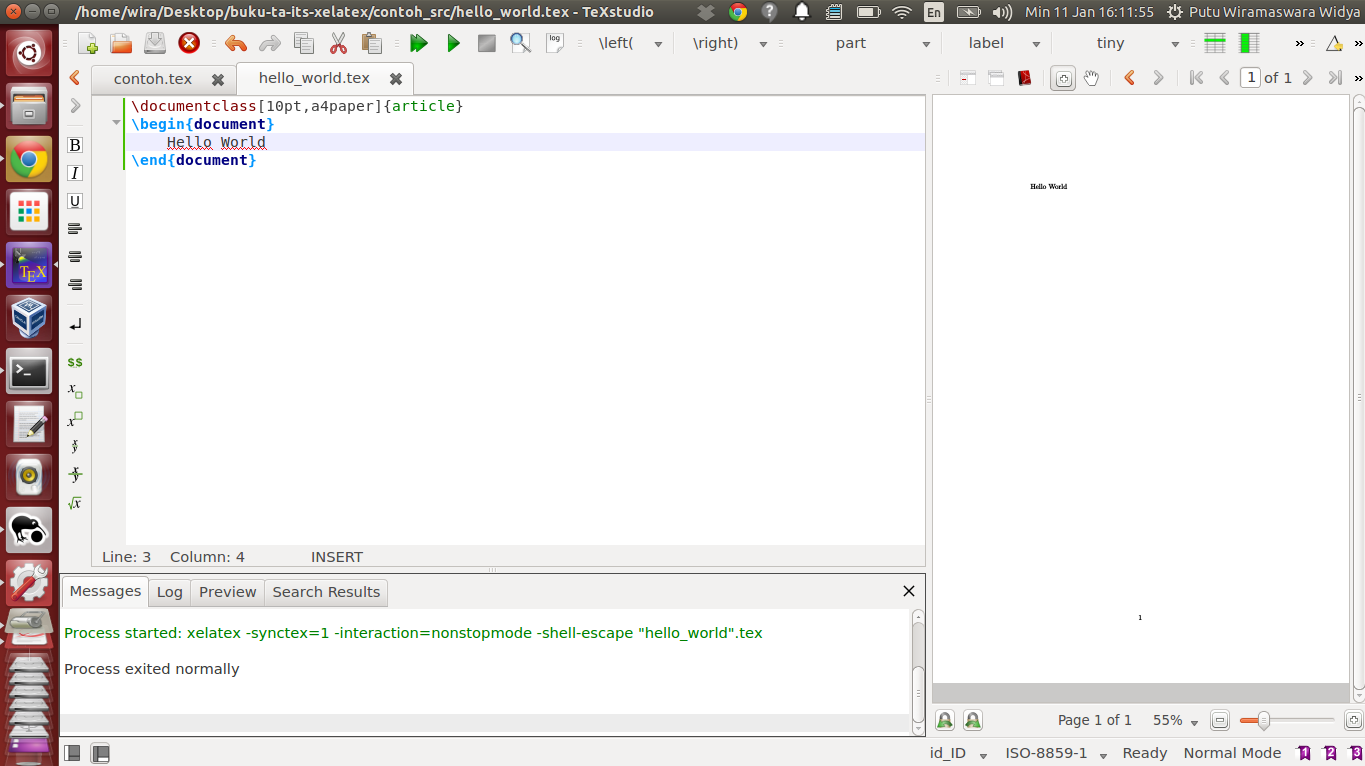
\includegraphics[width=\linewidth]{contoh_img/texstudio}
			\caption{Tangkapan Layar \TeX{}studio}
			\label{gambarTexStudio}
		\end{figure}

        Jika sudah siap, silahkan membuka teks editor favorit Anda dan mulai menulis beberapa bagian teks seperti pada Gambar \ref{kodeHelloWorld}. Anda boleh menggunakan atau tidak indentasi pada setiap elemen. Penggunaan indentasi dalam hal ini bermaksud untuk memudahkan pembacaan struktur dokumen. Simpan berkas tersebut ke dalam berkas bernama "hello\_world.tex".
        
        \begin{figure}[h]
	        \lstinputlisting[language=TeX]{contoh_src/hello_world.tex}
	        \caption{Artikel Hello World}
	        \label{kodeHelloWorld}
        \end{figure}
        
        \subsection{Kompilasi Dokumen}
        
        Untuk memroses kode ke dokumen, Anda dapat menggunakan menu \texttt{Tools | Build and View (F1)} pada \TeX{}studio atau memanggil perintah berikut pada antarmuka teks (jika Anda sudah terbiasa dan pastikan berada pada direktori yang tepat) :
        
        \texttt{latex hello\_world.tex}
        
        Setelah beberapa pesan kompilasi muncul, Anda dapat membuka berkas "hello\_world.dvi" yang merupakan dokumen hasil kompilasi.
        
        Jika Anda ingin membuat dokumen dalam format PDF, Anda dapat menggunakan kompilator bernama \texttt{pdflatex}. Hasilnya dapat dilihat pada Gambar \ref{gambarHelloWorldPDF} Kompilator bawaan dapat Anda ubah dalam \TeX{}studio melalui menu \texttt{Options | Configure TeX Studio | Build | Default Compiler}. Untuk lebih jelasnya, distribusi \TeX atau \LaTeX umumnya memiliki kompilator sebagai berikut :
        
        \begin{itemize}
	        \item \textbf{\LaTeX} merupakan kompilator bawaan untuk \LaTeX yang merupakan pengembangan dari \TeX{} (dikembangkan oleh Donald Knuth). Fitur utama \LaTeX{} antara lain: pilihan kelas dokumen dan adanya strukturisasi dokumen.
	        \item \textbf{pdf\LaTeX} merupakan pengembangan dari \LaTeX yang akan menghasilkan luaran dalam bentuk PDF ketimbang DVI.
	        \item \textbf{Xe\LaTeX} merupakan pengembangan dari \LaTeX dengan dukungan fonta berbasis TrueType. Templat Buku TA ini menggunakan Xe\LaTeX agar dapat menggunakan fonta \textbf{Times New Roman} bawaan dari Windows.
        \end{itemize} 
         
		\begin{figure}[h]
			\centering
			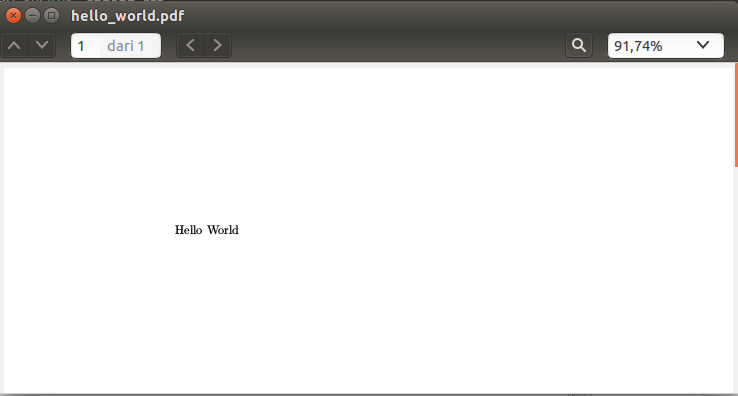
\includegraphics[width=\linewidth]{contoh_img/hello_world.pdf.png}
			\caption{hello\_world.pdf}
			\label{gambarHelloWorldPDF}
		\end{figure}
		
		\subsection{Struktur Kode \LaTeX}
		Secara umum, struktur kode berkas .tex dibagi menjadi dua bagian:
		
		\begin{itemize}
			\item \textbf{Preambule}, merupakan bagian yang berada sebelum \texttt{\textbackslash{}begin\{document\}} dilakukan. Pada bagian ini, biasanya diawali dengan deklarasi \texttt{\textbackslash{}documentclass} (dibahas selanjutnya) dan deklarasi impor paket tambahan yang dibutuhkan (melalui \texttt{\textbackslash{}usepackage\{\}}).
			\item \textbf{Dokumen} merupakan bagian yang diawali dengan \texttt{\textbackslash{}begin\{document\}} dan diakhiri dengan \texttt{\textbackslash{}end\{document\}}. Pada bagian inilah Anda mengisi konten dari dokumen Anda secara berurutan per halamannya.
		\end{itemize}
        
        \subsection{Kelas Dokumen Bawaan}
        
        Anda tidak seharusnya memikirkan bagaimana templat dan tata letak dokumen Anda di \LaTeX{} jika Anda memang fokus untuk menulis dokumen. Filosofi di \LaTeX{} menegaskan bahwa Anda memang harus fokus terhadap isi konten daripada terdistraksi dengan bagaimana wujud dokumen ketika dicetak. Untuk tujuan ini, \LaTeX{} beserta para komunitas menyediakan banyak templat untuk banyak keperluan yang bisa digunakan oleh pengguna sehingga mereka bisa langsung fokus mengisi konten dari dokumen mereka. Jenis templat ini dapat Anda pilih pada bagian \texttt{\textbackslash{}documentclass\{\textbf{nama-templat}\}}.
        
        \LaTeX{} sendiri memiliki beberapa templat bawaan :
        \begin{itemize}
        	\item \textbf{article}: templat untuk artikel ilmiah.
        	\item \textbf{book}: templat untuk penulisan buku, terdapat struktur dokumen layaknya buku seperti \texttt{part} dan \texttt{chapter}.
        	\item \textbf{report}: seperti templat \textbf{book} tapi tidak memiliki pembagian halaman awal, halaman isi dan lampiran.
        	\item \textbf{letter}: untuk penulisan dokumen tanpa struktur di dalamnya.
        	
        \end{itemize}
        Anda dapat menambahkan beberapa opsi pada templat yang Anda pilih dengan menambahkan argumen opsional (menggunakan kurung siku) pada deklarasi \texttt{\textbackslash{}documentclass}. Misalnya, jika Anda ingin membuat dokumen buku dengan ukuran kertas A5 dengan ukuran fonta 11pt (seperti Buku TA), Anda bisa membuat deklarasi sebagai berikut:
        
        \texttt{\textbackslash{}documentclass[a5paper,11pt]\{book\}}
        
        Selain templat bawaan \LaTeX, terdapat beberapa templat yang disediakan oleh komunitas:
        
        \begin{itemize}
        	\item \textbf{IEEEtran} merupakan templat untuk menulis jurnal dalam format IEEE. Bisa digunakan juga untuk pengiriman jurnal ilmiah POMITS. (Contoh pada Gambar \ref{gambarIEEEtran})
        	\item \textbf{beamer} merupakan templat untuk membuat \emph{slide} presentasi. (Contoh pada Gambar \ref{gambarBeamer})
        	\item \textbf{a0poster} merupakan templat untuk membuat dokumen dengan ukuran kertas yang besar, seperti poster.
        	\item \textbf{memoir} merupakan sekumpulan templat untuk kebutuhan penulisan buku fiksi maupun non-fiksi.
        	\item \textbf{moderncv} untuk penulisan Curriculum Vitae.
        	\item dan masih banyak lagi.
        \end{itemize}
        
        \begin{figure}[h]
        	\centering
        	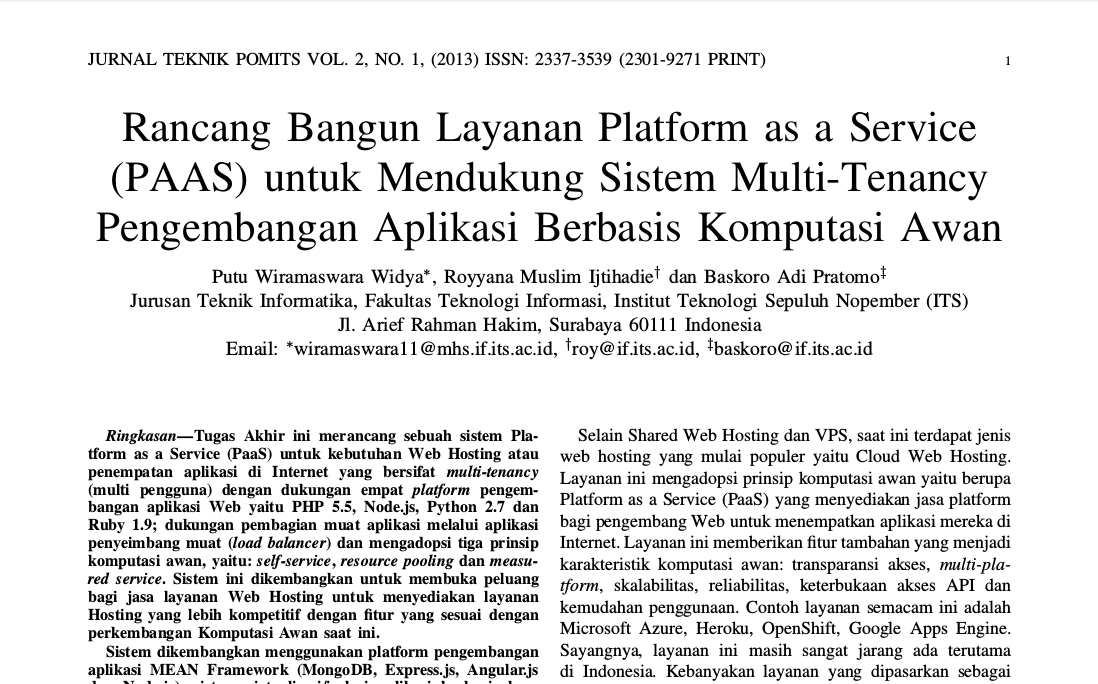
\includegraphics[width=\linewidth]{contoh_img/IEEETran}
        	\caption{Contoh penggunaan templat IEEETran}
        	\label{gambarIEEEtran}
        \end{figure}
        
        \begin{figure}[h]
        	\centering
        	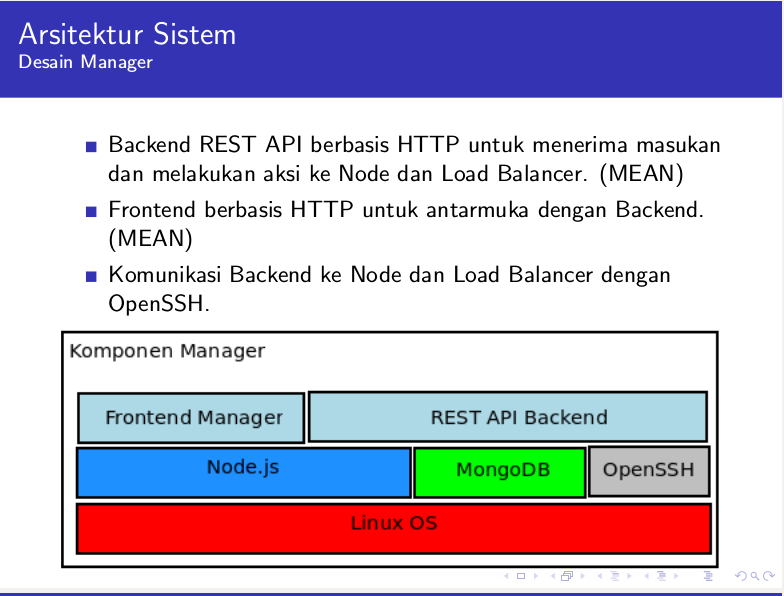
\includegraphics[width=\linewidth]{contoh_img/beamer}
        	\caption{Contoh penggunaan templat beamer}
        	\label{gambarBeamer}
        \end{figure}

        
        \section{Cara Menggunakan Templat \texttt{ta-its}}
        Berkas \texttt{ta-its.cls} yang disertakan pada templat ini merupakan bagian utama dari templat Buku TA ITS yang siap untuk digunakan. Untuk menggunakan templat ini, salinlah berkas \texttt{ta-its.cls} dan direktori \texttt{img/} (berisi berkas sampul) ke direktori di mana Anda akan menulis Buku TA Anda. Kemudian gunakan templat ini sebagai kelas dokumen melalui deklarasi sebagai berikut pada Preambule :
        
        \texttt{\textbackslash{}documentclass\{buku-ta\}}
        
        Templat ini tidak menerima argumen tambahan apapun untuk saat ini. Selanjutnya, Anda wajib mendeklarasikan Judul, Pengarang, Dosen dan Jurusan juga pada bagian Preambule. Formatnya adalah sebagai berikut :
        
        \begin{itemize}
        	\item \texttt{\textbackslash{}title\{Judul TA dalam Bahasa Indonesia\}\{Judul TA dalam Bahasa Inggris\}}
        	\item \texttt{\textbackslash{}author\{Nama Penulis\}\{NRP Penulis\}}
        	\item \texttt{\textbackslash{}degree\{Nama Gelar\}\{Bidang Studi\}\{Program Studi\}\{Jurusan\}\{Jurusan (English)\}\{Fakultas\}\{Fakultas Singkatan\}\{Fakultas (English)\}}
        	\item \texttt{\textbackslash{}time\{Bulan Pembuatan\}\{Tahun Pembuatan\}}
        \end{itemize}
        
        Kemudian pada bagian isi, templat ini menawarkan beberapa fungsi untuk pembuatan elemen buku secara otomatis, antara lain :
        
        \begin{itemize}
        	\item \texttt{\textbackslash{}maketitle} digunakan untuk membuat sampul dalam tiga halaman: Sampul Depan, Sampul Tengah, Sampul Tengah Bahasa Inggris.
        	\item \texttt{\textbackslash{}legalityPaper} untuk membuat halaman pengesahan.
        	\item Environment \texttt{abstrak} dan \texttt{abstract} untuk penulisan Abstrak dalam Bahasa Indonesia dan Inggris.
        \end{itemize}
        
        Contoh penggunaan dapat Anda lihat pada berkas \texttt{contoh.tex}.
        
        Dengan menggunakan templat ini, Anda akan menghemat waktu Anda untuk membuat sampul dan halaman pengesahan yang kadang bisa membuat kerepotan dalam hal pengaturan posisi indentasinya.
        
        \section{Struktur Dokumen \LaTeX{}}
        Dokumen \LaTeX{} terdiri dari struktur yang dibuat berdasarkan struktur dokumen sehari-hari. Sebagai penulis dokumen, Anda wajib menggunakan struktur ini sehingga \LaTeX{} dapat melakukan hal lain yang membantu Anda dalam mengorganisir dokumen seperti misalnya pembuatan Daftar Isi. Berikut adalah struktur dokumen yang ada di \LaTeX{} diurutkan berdasarkan hirarkinya.
        
        \begin{ltabulary}{|L|L|} % L = Rata kiri untuk setiap kolom, | = garis batas vertikal.
        	
        	% Kepala tabel, berulang di setiap halaman
        	\caption{Struktur hirarki dokumen \LaTeX{}} \label{tabelStrukturDokumen} \\
        	\hline
        	\textbf{Nama} & \textbf{Peruntukkan} \\ \hline
        	
        	\endhead
        	\endfoot
        	\endlastfoot
        	
        	% Isi Tabel
        	\textbf{\textbackslash{}part\{Judul Bagian\}} & \texttt{book} \\ \hline
        	\textbf{\textbackslash{}chapter\{Judul Bab\}} & \texttt{book} dan \texttt{report} \\ \hline
        	\textbf{\textbackslash{}section\{Judul Subbab\}} & semua kecuali \texttt{letter} \\ \hline
        	\textbf{\textbackslash{}subsection\{Judul Subsubbab\}} & semua kecuali \texttt{letter} \\ \hline
        	\textbf{\textbackslash{}subsubsection\{Judul Subsubsubbab\}} & semua kecuali \texttt{letter} \\ \hline
        	\textbf{\textbackslash{}paragraph\{Judul Paragraf\}} & semua\\ \hline
        	
        \end{ltabulary}
        
        Untuk templat pihak ketiga, Anda dapat melihat dokumentasi dari templat bersangkutan. Sebagai informasi, templat \texttt{ta-its} dibuat berdasarkan templat \texttt{book} sehingga struktur dokumennya sama.
        
        \section{Paragraph dan Teks}
        \section{Daftar}
        \section{Gambar}
        \section{Tabel}
        \section{Rumus Matematika}
        \section{Algoritma}
        \section{Kode Sumber}
        

\appendix % Halaman lampiran, dengan judul LAMPIRAN X

\backmatter % Lampiran tanpa judul LAMPIRAN X, biasanya untuk BIODATA PENULIS
\end{document}
